\documentclass[german,10pt,a4paper,twocolumn,colorscheme=darkblue]{orarticle}
\usepackage{epstopdf}

		
% ****************************************************************************** %
% ******************************** DOCUMENT ************************************ %
% ****************************************************************************** %
\begin{document}

%	\subject{Quick Manual}
	\title{Scarlet Gamma Manual}
	\authors{Johannes Jendersie, David Kuri, Florian Uhde}
	\abstract{Einführung}{
		Scarlet Gamma ist eine Pen \& Paper Plattform, die es ermöglicht in Echtzeit auf die Welt und die Spieleraktionen zu reagieren und alles zu verändern. Zum Beispiel ist es möglich Dungeons zu verändern, neue Räume und sogar neue Gegnertypen zu jedem Zeitpunkt einzuführen. Einige Aktionen wie das Kampfsystem sind auf das Pathfinder (D\&D) Regelwerk ausgelegt. Es ist aber auch möglich das Tool für andere Spielrunden einzusetzen. Dieses Dokument bietet eine Übersicht über die Funktionsweise und die wichtigsten Aktionen.
	}
	\maketitle

	\tableofcontents
	
	\section{Spieler und Meister}
		Wie bei normalen P\&P Runden übernimmt ein Spieler die Rolle des Spielleiters welcher absolute Macht hat. Dieser stellt auch den Server für das Spiel.
	
		\subsection{Neue Welten}
			Wählt man im Hauptmenü 'Launch' so wird der Server gestartet. In jedem Fall muss eine Welt geladen oder erstellt werden. Soll ein Abenteuer fortgesetzt werden muss der Name der existierenden Datei eingegeben werden. Andernfalls kann ein neuer Name gewählt und "Erstellen" gedrückt werden. Achtung: Dies überschreibt Welten, wenn die Datei bereits existierte.
			
			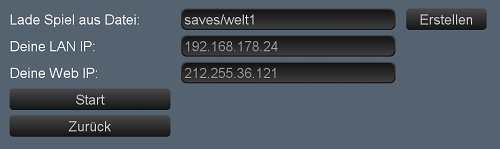
\includegraphics[width=\linewidth]{img/launch}
			
			Je nach dem ob Spieler sich im LAN oder über das Internet einloggen möchten sollten eine oder beide IP-Adressen notiert werden um sie den Spielern mitzuteilen, sobald die Welt geladen wurde.
			
		\subsection{Spielvorbereitung}
			Ähnlich der normalen Vorbereitung auf Papier sollte der Spielleiter die Welt für das Abenteuer planen und bauen. Dazu kann er nach dem Serverstart einfach neue Objekte und Karten erstellen wobei in dieser Zeit kein Spieler eingeloggt ist. Zusätzliche Vorbereitung auf Papier sind dabei möglich. Um Texte für NSCs zu schreiben empfiehlt es sich dies in Extra-Textdateien zu speichern und später an den entsprechenden Stellen in den Chat einzufügen.
		
		\subsection{Einem Spiel beitreten}
			Nach wählen der Option 'Spiel beitreten' im Hauptmenü muss eine Verbindung zum gestarteten Server hergestellt werden. Welche IP-Adresse dieser hat wird beim Starten des Servers angezeigt.
			
			Es kann passieren, dass eine Firewall die Verbindung verhindert. Dann muss eine entsprechende Regel für Scarlet Gamma hinzugefügt werden. Im Spiel über das Internet ist außerdem darauf zu achten, dass der Port 42961 freigegeben ist.
			
			Anschließend wird die Welt übertragen und eine Liste mit existierenden Spielern darin angezeigt. Wird eine Abenteuer fortgesetzt reicht ein Klick. In einer neuen Welt oder wenn ein neuer Charakter hinzukommt kann dieser über 'Neuer Spieler' erstellt werden.
		
	\section{Komponentenbasiertes Objektsystem}
		Alles in der Welt folgt dem gleichen Schema um ein größtmögliche Kombinationsvielfalt zu ermöglichen.
		
		- Erklärung PropertyPanel
	
		\subsection{Besondere Eigenschaften}
	
	\section{Editor}
		- Erklärung der ganzen Master Tools
	
	\section{Der Spielfluss}
	
		\subsection{Pause}
		\subsection{Kämpfe}
			\subsubsection{Subsub}
			
	\section{Shortcuts}
		Im folgenden ist die Tastaturbelegung aufgelistet. [M] bedeutet, dass die Aktion im Master-Modus, also dem Spielleiter zur Verfügung steht. [S] bedeutet entsprechend, dass der Spieler die Aktion ausführen kann.
		\begin{description}
			\item[C] [M,S] öffnet den Charakterbildschirm für das ausgewählte Objekt (M) oder den Spieler.
			\item[Alt+1 ... Alt+0] [M] Ändere Sichtbarkeit der Layer 1 - 10
			\item[Alt] Blende alle Layer wieder ein.
		\end{description}
	
	
\end{document}